% !TeX program = pdflatex
\documentclass[border=6pt]{standalone}
\usepackage{tikz}
\usetikzlibrary{arrows.meta, positioning, calc}

\definecolor{MediumRed}{rgb}{0.925, 0.345, 0.345}
\definecolor{MediumGreen}{rgb}{0.37, 0.7, 0.66}
\definecolor{MediumBlue}{rgb}{0.015, 0.315, 0.45}
\definecolor{DarkBlue}{rgb}{0.05, 0.15, 0.35}

\begin{document}
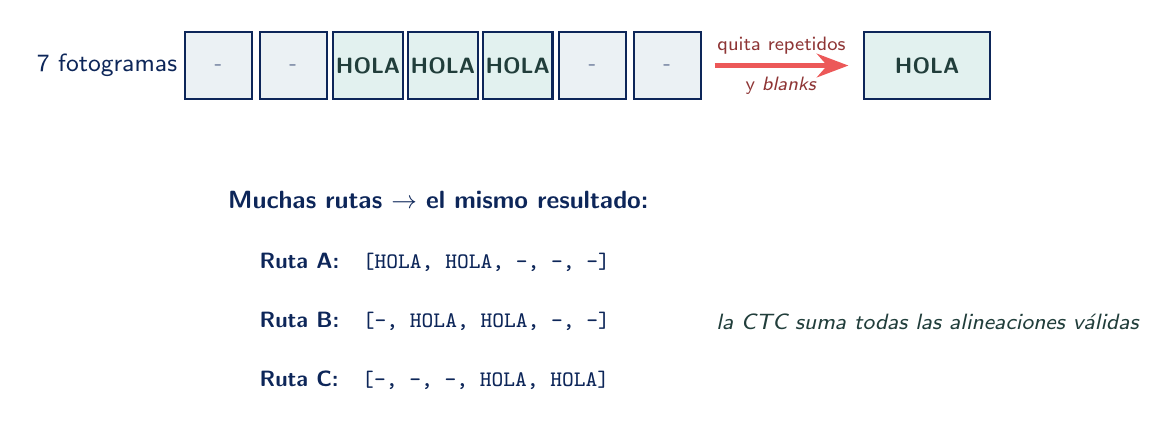
\begin{tikzpicture}[
    font=\sffamily,
    frame/.style={draw=DarkBlue, thick, minimum size=0.85cm, inner sep=1pt,
        font=\sffamily\footnotesize\bfseries},
    blank/.style={frame, fill=MediumBlue!8, text=DarkBlue!55},
    sign/.style={frame, fill=MediumGreen!18, text=MediumGreen!35!black},
]

% ---- secuencia por fotograma ----
\node[font=\sffamily\small, text=DarkBlue, anchor=east] at (-0.4,0) {7 fotogramas};
\foreach \i/\lbl/\ty in {0/{-}/blank,1/{-}/blank,2/HOLA/sign,3/HOLA/sign,4/HOLA/sign,5/{-}/blank,6/{-}/blank}
    \node[\ty] (f\i) at (\i*0.95,0) {\lbl};

% ---- colapso ----
\draw[-{Stealth[length=4mm]}, line width=1.6pt, MediumRed]
    (6.3,0) -- node[above, font=\sffamily\scriptsize, text=MediumRed!60!black]
    {quita repetidos} node[below, font=\sffamily\scriptsize, text=MediumRed!60!black]
    {y \emph{blanks}} (8.0,0);
\node[sign, minimum width=1.6cm] at (9.0,0) {HOLA};

% ---- rutas validas ----
\node[font=\sffamily\small\bfseries, text=DarkBlue, anchor=west] at (0,-1.7)
    {Muchas rutas $\rightarrow$ el mismo resultado:};
\foreach \r/\seq/\y [count=\j] in {%
    A/{HOLA, HOLA, -, -, -}/-2.5,
    B/{-, HOLA, HOLA, -, -}/-3.25,
    C/{-, -, -, HOLA, HOLA}/-4.0}{
    \node[font=\sffamily\footnotesize, text=DarkBlue, anchor=west] at (0.4,\y)
        {\textbf{Ruta \r:}\quad \texttt{[\seq]}};
}
\node[font=\sffamily\footnotesize\itshape, text=MediumGreen!35!black, anchor=west] at (6.2,-3.25)
    {la CTC suma todas las alineaciones válidas};

\end{tikzpicture}
\end{document}
